\chapter{CHIP-8}
\label{chap:ch3}

\section{About}
\label{sec:ch3sec1}

\par CHIP-8, sometimes spelled as CHIP8, is a programming language and virtual machine specification developed by Joseph Weisbecker on the 1802 processor of the COSMAC VIP computer in the mid-1970s.

\par It was meant to be an educational tool mainly designed around creating simple video games with much more ease and less resources than conventional programming languages of the time such as BASIC.

\par Even today it is widely used as an introduction for people that are taking up software emulation as a programming hobby because of its simplicty and ease of implementation.

\vspace{1cm}

\begin{minipage}{\linewidth}
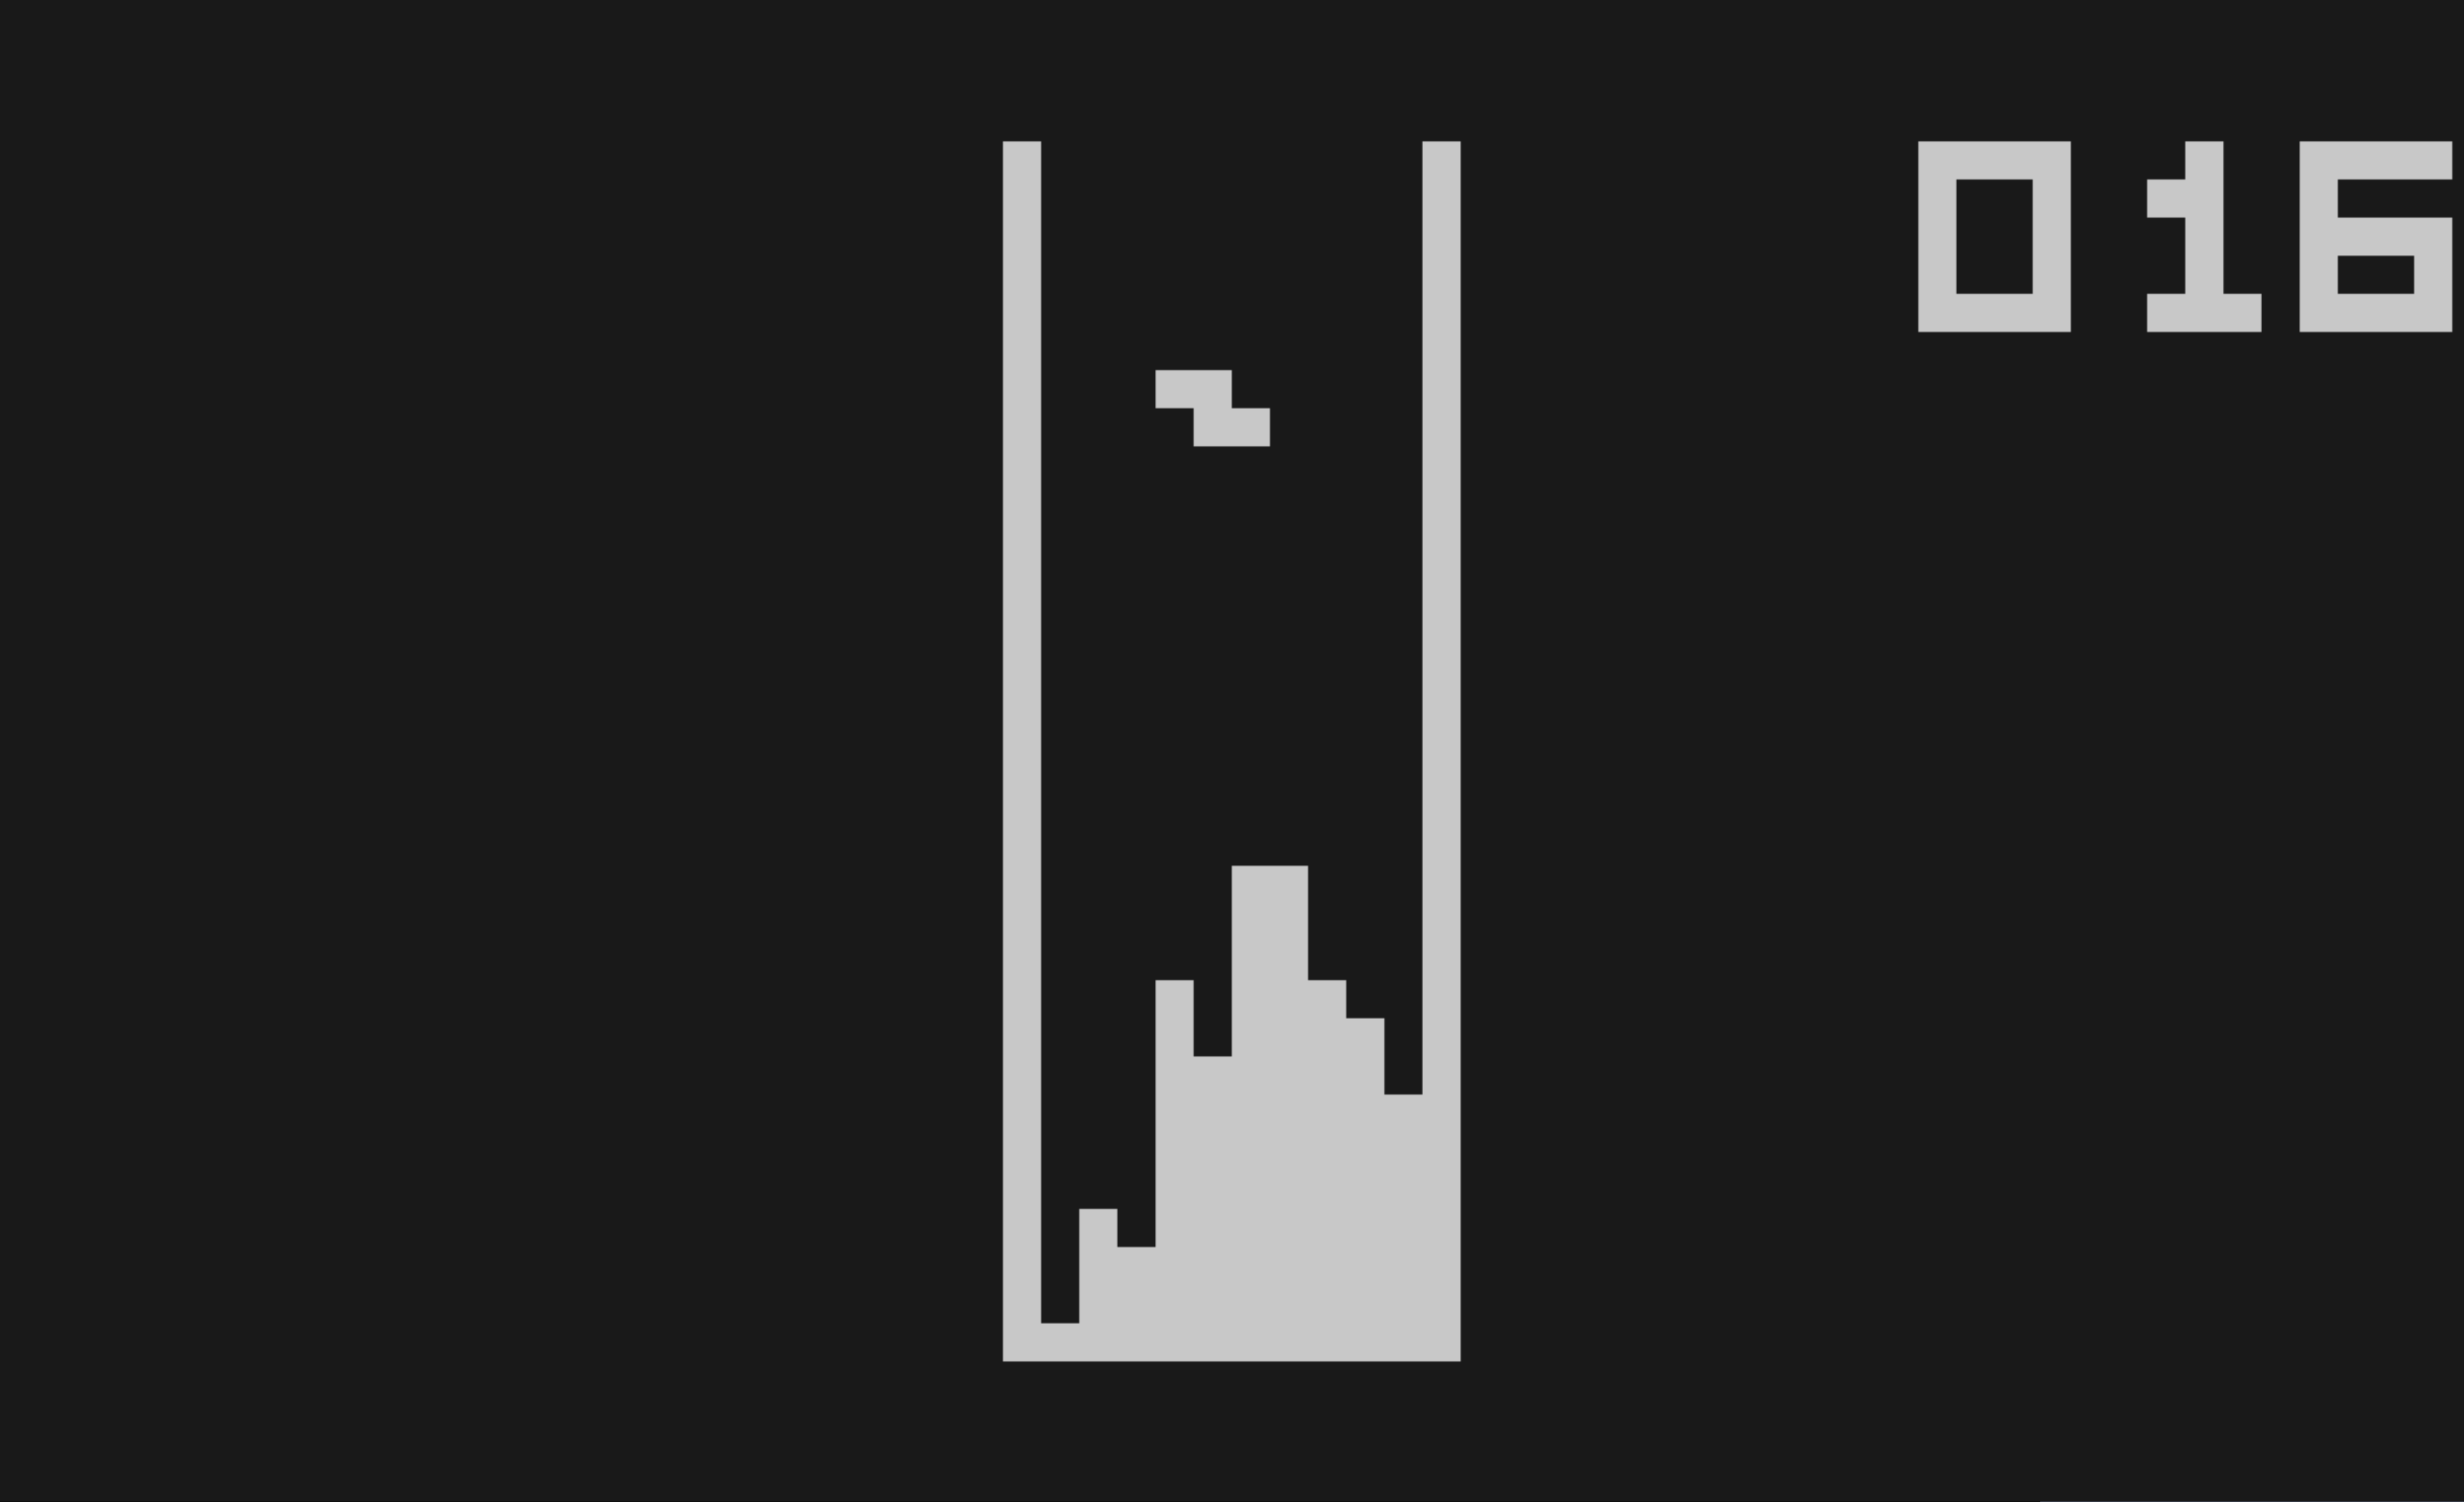
\includegraphics[width=\textwidth]{tetris_ch8}
\captionof{figure}{Tetris clone written in CHIP-8 by Fran Dachille in 1991 running in \href{https://github.com/solomonarul/edra}{\texttt{Edra}}.}
\end{minipage}

\clearpage

\section{Virtual machine description}
\label{sec:ch3sec2}

\subsubsection{Memory}

\par The CHIP-8 virtual machine provides \textit{4KB} of accessible memory, reflecting the addressable range of its 16-bit memory registers. An exception to this is the \texttt{I} register, primarily utilized for drawing and memory operations, which is implemented as a 12-bit register rather than 16-bit. Multi-byte data within the system is stored in big-endian format, meaning the most significant byte precedes the least significant byte in memory.

\par Historically, the virtual machine's memory space overlapped with that of the interpreter, resulting in programs typically being loaded starting at address \texttt{0x200}. In contemporary implementations, this memory region is often repurposed to store font data, as emulators maintain separate memory spaces for code and data.

\par Furthermore, the uppermost \textit{256} bytes of memory (addresses \texttt{0xF00}-\texttt{0xFFF}) were originally allocated for display data. The adjacent lower segment (addresses \texttt{0xEA0}-\texttt{0xEFF}) was reserved for the interpreter's internal use, including the call stack and various system variables, though this reservation is frequently disregarded in modern emulator designs where the display data and emulator implementation is stored in a separate memory location.

\subsubsection{Registers}

\par The CHIP-8 virtual machine contains \textit{16} general-purpose 8-bit registers, labeled \texttt{V0} through \texttt{VF}. The \texttt{VF} register is reserved for use as a flag by certain instructions and should generally be avoided for storing general data, as its value may be altered implicitly during execution.

\subsubsection{Display}

\par The CHIP-8 display operates at a resolution of \texttt{64x32} pixels, rendering graphics in monochrome. Sprites are rendered onto the screen using a bitwise XOR based drawing method, whereby the sprite pixels are bitwise XORed with the existing framebuffer content. This technique allows for simple sprite toggling and erasure.

\par Additionally, the interpreter sets the flag register \texttt{VF} to \textit{1} if any pixel collision occurs during this process, specifically when a pixel is turned off as a result of overlapping pixels, providing a mechanism for collision detection in games and applications.

\begin{table}[H]
\centering
\begin{tabular}{
>{\columncolor[HTML]{333333}}l 
>{\columncolor[HTML]{333333}}l 
>{\columncolor[HTML]{333333}}l lllll
>{\columncolor[HTML]{EFEFEF}}l 
>{\columncolor[HTML]{EFEFEF}}l 
>{\columncolor[HTML]{EFEFEF}}l l
>{\columncolor[HTML]{333333}}l l
>{\columncolor[HTML]{333333}}l }
    &                          &  &  &  &                          &  &  &  &  &  &  &  & \cellcolor[HTML]{333333} &  \\
    & \cellcolor[HTML]{EFEFEF} &  &  &  & \cellcolor[HTML]{333333} &  &  &  &  &  &  &  &                          &  \\
\cellcolor[HTML]{EFEFEF} &
    &
    \cellcolor[HTML]{EFEFEF} &
    &
    \cellcolor[HTML]{333333} &
    \cellcolor[HTML]{333333} &
    \cellcolor[HTML]{333333} &
    &
    \cellcolor[HTML]{333333} &
    \cellcolor[HTML]{333333} &
    \cellcolor[HTML]{333333} &
    &
    &
    &
    \\
    & \cellcolor[HTML]{EFEFEF} &  &  &  & \cellcolor[HTML]{333333} &  &  &  &  &  &  &  &                          &  \\
    &                          &  &  &  &                          &  &  &  &  &  &  &  & \cellcolor[HTML]{333333} & 
\end{tabular}
\caption{Illustration of sprite XOR-ing, transforming an 8 (left) into a 0 (right), \texttt{VF} is set in this case to \textit{1}. The \textit{+} sign is not part of the sprite.}
\end{table}

\par The CHIP-8 virtual machine includes two timers: the delay timer and the sound timer. Both decrement at a fixed rate of \textit{60hz}. While the delay timer is typically used for timing-related logic within programs, the sound timer serves as an audio trigger. When the sound timer holds a non-zero value, it indicates that a sound should be produced.

\par The exact characteristics of the sound are not formally specified in the original CHIP-8 documentation, leaving its implementation to the discretion of the emulator developer. The most commonly adopted convention is to emulate the sound as a simple buzzer tone, consistent with the limitations of the original hardware.

\subsubsection{Input}

\par Input on the CHIP-8 system is handled via a hexadecimal keypad consisting of \textit{16} keys, labeled with values ranging from \textit{0} to \textit{F}.

\par A common convention is to arrange the keys in a 4 by 4 grid that mirrors the original layout, allowing intuitive input translation between physical keyboards and the virtual machine environment:

\begin{table}[H]
\centering
\begin{tabular}{| c | c | c | c |}
\hline
1 & 2 & 3 & C \\ \hline
4 & 5 & 6 & D \\ \hline
7 & 8 & 9 & E \\ \hline
A & 0 & B & F \\ \hline
\end{tabular}
\caption{Original input layout on the COSMAC VIP}
\end{table}

\begin{table}[H]
\centering
\begin{tabular}{| c | c | c | c |}
\hline
1 & 2 & 3 & 4 \\ \hline
Q & W & E & R \\ \hline
A & S & D & F \\ \hline
Z & X & C & V \\ \hline
\end{tabular}
\caption{Commonly used layout on modern keyboards}
\end{table}

\subsubsection{Instructions}

\begin{longtable}{|c|c|p{9cm}|}
\hline
\textbf{Opcode} & \textbf{Mnemonic} & \textbf{Description} \\
\hline
\endfirsthead

\hline
\textbf{Opcode} & \textbf{Mnemonic} & \textbf{Description} \\
\hline
\endhead

\hline
\endfoot

\hline
\endlastfoot

00E0 & CLS & Clear the display. \\
00EE & RET & Return from a subroutine. \\
1NNN & JP addr & Jump to location NNN. \\
2NNN & CALL addr & Call subroutine at NNN. \\
3XNN & SE Vx, byte & Skip next instruction if Vx is equal to NN. \\
4XNN & SNE Vx, byte & Skip next instruction if Vx is not equal to NN. \\
5XY0 & SE Vx, Vy & Skip next instruction if Vx is equal to Vy. \\
6XNN & LD Vx, byte & Set Vx = NN. \\
7XNN & ADD Vx, byte & Set Vx = Vx + NN. \\
8XY0 & LD Vx, Vy & Set Vx = Vy. \\
8XY1 & OR Vx, Vy & Set Vx = Vx OR Vy. \\
8XY2 & AND Vx, Vy & Set Vx = Vx AND Vy. \\
8XY3 & XOR Vx, Vy & Set Vx = Vx XOR Vy. \\
8XY4 & ADD Vx, Vy & Set Vx = Vx + Vy, set VF = carry. \\
8XY5 & SUB Vx, Vy & Set Vx = Vx - Vy, set VF = NOT borrow. \\
8XY6 & SHR Vx {, Vy} & Set Vx = Vx SHR 1. \\
8XY7 & SUBN Vx, Vy & Set Vx = Vy - Vx, set VF = NOT borrow. \\
8XYE & SHL Vx {, Vy} & Set Vx = Vx SHL 1. \\
9XY0 & SNE Vx, Vy & Skip next instruction if Vx is not equal to Vy. \\
ANNN & LD I, addr & Set I = NNN. \\
BNNN & JP V0, addr & Jump to location NNN + V0. \\
CXNN & RND Vx, byte & Set Vx = random byte AND NN. \\
DXYN & DRW Vx, Vy, nibble & Display n-byte sprite starting at memory location I at (Vx, Vy), set VF = collision. \\
EX9E & SKP Vx & Skip next instruction if key with the value of Vx is pressed. \\
EXA1 & SKNP Vx & Skip next instruction if key with the value of Vx is not pressed. \\
FX07 & LD Vx, DT & Set Vx = delay timer value. \\
FX0A & LD Vx, K & Wait for a key press, store the value of the key in Vx. \\
FX15 & LD DT, Vx & Set delay timer = Vx. \\
FX18 & LD ST, Vx & Set sound timer = Vx. \\
FX1E & ADD I, Vx & Set I = I + Vx. \\
FX29 & LD F, Vx & Set I = location of sprite for digit Vx. \\
FX33 & LD B, Vx & Store BCD representation of Vx in memory locations I, I+1, and I+2. \\
FX55 & LD [I], Vx & Store registers V0 through Vx in memory starting at location I. \\
FX65 & LD Vx, [I] & Read registers V0 through Vx from memory starting at location I. \\
\end{longtable}

\par The original CHIP-8 implementation supported a total of 35 instructions, although only 31 were explicitly documented in the initial specification. Notably, opcodes such as \texttt{8XY3}, \texttt{8XY6}, \texttt{8XY7}, and \texttt{8XYE} were omitted from the formal documentation.

\par This omission is likely attributable to the historical context of CHIP-8’s design, which was implemented atop the RCA 1802 microprocessor. The \texttt{8XY*} instruction group closely mirrors operations available in the 1802’s Arithmetic Logic Unit (ALU), suggesting that these opcodes may have originated from the hardware's native capabilities rather than being explicitly defined by the CHIP-8 interpreter itself.

\par Subsequent extensions to the CHIP-8 instruction set, such as those introduced in SCHIP (Super CHIP) and other variants, have redefined or augmented the behavior of certain instructions. For example, instructions \texttt{FX55} and \texttt{FX65} originally incremented the index register \texttt{I} after each memory write or read, respectively. However, later implementations, including SCHIP, omit this side effect, reflecting divergence in interpretation and a lack of standardization across extensions, which will be discussed later.

\section{Emulator implementation}
\label{sec:ch3sec3}

\par The core CHIP-8 library, \href{https://github.com/solomonarul/cchip8}{\texttt{cchip8}}, is organized into modular components: the state, the interpreter, and the static compiler. This architecture enforces a clear separation of concerns, where only the execution runners depend on the state module, and each module operates independently, promoting maintainability and extensibility.

\par The state module, defined in \href{https://github.com/solomonarul/cchip8/blob/main/inc/cchip8/state.h}{\texttt{state.h}}, functions as the central interface between the emulator core and the external environment. It encapsulates the full virtual machine state as well as a set of callback function pointers that enable host-controlled behavior, such as memory access, rendering, input handling, and random number generation.

\par The \texttt{chip8\_state}'s structure maintains essential CHIP-8 runtime components, including program counter (\texttt{pc}), index register (\texttt{i}), stack and stack pointer (\texttt{stack}, \texttt{sp}), \textit{16} general-purpose registers (\texttt{v[0x10]}), timers (\texttt{dt}, \texttt{st}), display resolution parameters, and font memory addresses.

\par In addition, it includes a flag \texttt{draw\_flag} for screen redraw signaling and a variable \texttt{last\_key} to track the most recently pressed key to emulate accurate behaviour for the \textit{FX0A} instruction family.

\par The embedded function pointers (\texttt{read\_b}, \texttt{read\_w}, \texttt{write\_b}, etc.) abstract interactions with the host system. These allow the emulator to delegate low-level operations such as I/O, drawing, screen clearing, input polling, and random number generation to external implementations, facilitating portability and customization.

\par An auxiliary argument pointer (\texttt{aux\_arg}) is also provided to pass user-defined data to these callbacks, supporting more complex execution contexts if needed.

\begin{minted}[
    linenos,                % add line numbers
    fontfamily=tt,          % typewriter font
    fontsize=\small,        % size
    breaklines,             % allow line breaks
    tabsize=4               % size of tab
]{C}
struct chip8_state
{
    bool draw_flag;
    chip8_run_mode_t mode;
    uint16_t pc, i, stack[0x100];
    uint8_t display_width, display_height;
    uint8_t v[0x10], sp, dt, st, last_key;
    uint16_t lowres_font_address, hires_font_address;
    
    // Callbacks.
    chip8_read_b_f read_b;
    chip8_read_w_f read_w;
    chip8_write_b_f write_b;
    chip8_draw_sprite_f draw_sprite;
    chip8_clear_f clear_screen;
    chip8_key_status_f get_key_status;
    chip8_random_f get_random;
    chip8_resize_f resize;
    chip8_scroll_f scroll;
    
    void* aux_arg;  // Used for passing data to the callbacks.
};
\end{minted}

// TODO: proofread from here.

\subsection{Interpreter}
\label{subsec:ch3sec3sub1}

\par The interpreter, as defined in \href{https://github.com/solomonarul/cchip8/blob/main/inc/cchip8/cpu/interpreter.h}{\texttt{cpu/interpreter.h}}, encapsulates a minimal runtime structure responsible for controlling instruction execution.

\par The \texttt{chip8\_interpreter\_t} struct maintains three key fields: a boolean flag \texttt{running} to indicate whether the interpreter is actively executing instructions, a \texttt{long} field \texttt{timer} to track internal timing mechanisms, and a pointer \texttt{state} to the shared \texttt{chip8\_state\_t} structure, which contains the core emulator state.

\par This design ensures that the interpreter remains lightweight, delegating system-wide responsibilities to the state module while managing control flow and timing locally, and such, enables the interpreter to operate independently of the underlying platform or user interface, facilitating reuse and testing.

\begin{minted}[
    linenos,                % add line numbers
    fontfamily=tt,          % typewriter font
    fontsize=\small,        % size
    breaklines,             % allow line breaks
    tabsize=4               % size of tab
]{C}
struct chip8_interpreter
{
    bool running;
    long timer;
    chip8_state_t* state;
};
typedef struct chip8_interpreter chip8_interpreter_t;
\end{minted}

\par The function \texttt{chip8\_interpreter\_step(chip8\_interpreter\_t* self)} is responsible for executing a single instruction cycle within the interpreter. It represents the core of the CHIP-8 execution loop, fetching the current instruction from memory, decoding it, and dispatching it for execution.

\par Internally, instruction decoding is implemented using a large \texttt{switch} statement, a common pattern in interpreter design. The instruction opcode, 16 bits in CHIP-8, is fetched from memory using the program counter (\texttt{pc}) and then used to determine which operation to execute.

\par Each \texttt{case} in the \texttt{switch} corresponds to a specific opcode or opcode pattern, allowing for structured, readable, and performant instruction handling.

\par This dispatch method, while straightforward, also benefits from modern compiler optimizations that often convert large \texttt{switch} statements into jump tables, providing relatively fast execution times.

\par Additionally, this layout makes it easier to maintain and extend the interpreter, as new opcodes can be added with minimal structural disruption.

\section{Quirks and extensions}
\label{sec:ch3sec4}

\subsection{Modern Super CHIP-8}
\label{subsec:ch3sec4sub1}

\begin{minipage}{\linewidth}

\includegraphics[width=\textwidth]{octogon_ch8}
\captionof{figure}{Octogon by John Earnest running in \href{https://github.com/solomonarul/edra}{\texttt{Edra}}'s modern SCHIP mode.\\}
\end{minipage}

\par Lorem ipsum dolor sit amet, consectetur adipiscing elit, sed do eiusmod tempor incididunt ut labore et dolore magna aliqua. Ut enim ad minim veniam, quis nostrud exercitation ullamco laboris nisi ut aliquip ex ea commodo consequat. Duis aute irure dolor in reprehenderit in voluptate velit esse cillum dolore eu fugiat nulla pariatur. Excepteur sint occaecat cupidatat non proident, sunt in culpa qui officia deserunt mollit anim id est laborum

\section{Testing}
\label{sec:ch3sec5}

\par The current implementation has been tested for correctness using \href{https://github.com/Timendus/chip8-test-suite}{\texttt{Timendus' CHIP8 test suite}}, a well known test suite in the community. It assures correct behaviour, identical to the original implementation unless otherwise specified. 

\par The suite supports tests from the smallest subset of the instructions that could be implemented, enough for an image of the IBM logo to be displayed:

\begin{longtable}{|c|l|}
\hline
\textbf{Opcode} & \textbf{Description} \\ \hline
\endfirsthead

\hline
\textbf{Opcode} & \textbf{Description} \\ \hline
\endhead

\hline
\endfoot

\hline
\endlastfoot

00E0 & Clear the screen.                                        \\ \hline
6XNN & Load normal register with immediate value.               \\ \hline
ANNN & Load index register with immediate value.                \\ \hline
7XNN & Add immediate value to normal register.                  \\ \hline
DXYN & Draw sprite to screen (unaligned, easier to implement).  \\ \hline
1NNN & Jump (optional, only at the end).                        \\
\end{longtable}
// TODO: insert images here.

\par To the entire instruction set and the correct hardware timings and quirks, including the flags set by the instructions:

// TODO: insert images here.

\par These tests have been ran manually in all possible configurations to make sure the emulator is behaving as expected, even in modern SCHIP mode.

// TODO: insert images here.